% \documentclass[12pt, twoside]{article}
\usepackage[letterpaper, margin=1in, headsep=0.2in]{geometry}
\setlength{\headheight}{0.6in}
%\usepackage[english]{babel}
\usepackage[utf8]{inputenc}
\usepackage{microtype}
\usepackage{amsmath}
\usepackage{amssymb}
%\usepackage{amsfonts}
\usepackage[nomessages]{fp} %\FPeval{\var-name}{2*sin(pi/6)}
\usepackage{siunitx} %units in math. eg 20\milli\meter
\usepackage{yhmath} % for arcs, overparenth command
\usepackage{tikz} %graphics
\usetikzlibrary{quotes, angles, arrows, arrows.meta}
\usepackage{graphicx} %consider setting \graphicspath{{images/}}
\usepackage{parskip} %no paragraph indent
\usepackage{enumitem}
\usepackage{multicol}
\usepackage{venndiagram}

\usepackage{fancyhdr}
\pagestyle{fancy}
\fancyhf{}
\renewcommand{\headrulewidth}{0pt} % disable the underline of the header
\raggedbottom
\hfuzz=2mm %suppresses overfull box warnings

\usepackage{hyperref}

\fancyhead[LE]{\thepage}
\fancyhead[RO]{\thepage \\ Name: \hspace{4cm} \,\\}
\fancyhead[LO]{BECA / Dr. Huson / Geometry\\*  Unit 6: Analytic geometry\\* 28 November 2022}

\begin{document}

\subsubsection*{6.4 Classwork: Parallel and perpendicular slopes}
The slope of a line: $\displaystyle m=\frac{y_2-y_1}{x_2-x_1}$
\begin{enumerate}
\item Do Now: Given $\overleftrightarrow{PQ}$, $P(1,6)$, $Q(3,2)$. Find its slope, $y$-intercept, and equation.
\begin{flushright}
  \begin{tikzpicture}[scale=.65]
    \draw [help lines] (0,0) grid (7,9);
    \draw [thick, ->] (0,0) -- (7.4,0) node [below right] {$x$};
    \draw [thick, ->] (0,0)--(0,9.4) node [right] {$y$};
    \foreach \x in {1,...,7}
    \draw[shift={(\x,0)}] (0pt,-3pt)--(0pt,3pt) node[below=5pt] {$\x$};
    \foreach \y in {1,...,9}
    \draw[shift={(0,\y)}] (-3pt,0pt)--(3pt,0pt) node[left=5pt] {$\y$};
    \draw [thick, <->] (-0.25,8.5)--(4.25,-0.5);
    \draw [fill] (1,6) circle [radius=0.08] node[above right] {$P$};
    \draw [fill] (3,2) circle [radius=0.08] node[above right] {$Q$};
  \end{tikzpicture}
  \end{flushright}
  
\subsubsection*{Parallel lines have the same slope}
\item The line $l$ is shown on the grid below.
\begin{multicols}{2}
\begin{enumerate}
  \item Write down it's slope, $y$-intercept.\\ $m=$
  \hspace{2cm} $b=$
  \vspace{0.25cm}
  \item Write down the equation of line $l$.
  \vspace{1cm}
  \item Draw a line parallel to line $l$ though point $S$.
  \item Write down the equation of the second line.
\end{enumerate}
  \begin{center}
  \begin{tikzpicture}[scale=0.7]
    \draw [help lines] (-1,-1) grid (7,6);
    \draw [thick, ->] (-1.2,0) -- (7.4,0) node [below right] {$x$};
    \draw [thick, ->] (0,-1.2)--(0,6.4) node [right] {$y$};
    \foreach \x in {1, ..., 7} \draw (\x cm,1pt) -- (\x cm,-1pt) node[anchor=north] {$\x$};
    \foreach \y in {1,...,6} \draw (1pt,\y cm) -- (-1pt,\y cm) node[anchor=east] {$\y$};
    \draw [thick, <->] (-1.5,3.5) -- (6.6,6.2) node[above]{$l$};
    \fill (0,2) circle[radius=0.1] node[below right]{$S$};
  \end{tikzpicture}
  \end{center}
\end{multicols}\vspace{0.5cm}

\item The line has the equation $y=-x+7$. 
\begin{enumerate}
  \item Write down it's slope and $y$-intercept. \hspace{2cm} $m=$
  \hspace{2cm} $b=$
  \item Is the point $(4, 4)$ on the line? Justify your answer.
\end{enumerate}
\vspace{2cm}

\item The line $l$ is shown on the grid below.
\begin{multicols}{2}
\begin{enumerate}
  \item Write down it's slope, $y$-intercept.\\ $m=$
  \hspace{2cm} $b=$
  \vspace{0.25cm}
  \item Write down the equation of line $l$.
  \vspace{1cm}
  \item Draw a line parallel to line $l$ though point $S$.
  \item Write down the equation of the second line.
\end{enumerate}
  \begin{center}
  \begin{tikzpicture}[scale=0.7]
    \draw [help lines] (-1,-1) grid (7,6);
    \draw [thick, ->] (-1.2,0) -- (7.4,0) node [below right] {$x$};
    \draw [thick, ->] (0,-1.2)--(0,6.4) node [right] {$y$};
    \foreach \x in {1, ..., 7} \draw (\x cm,1pt) -- (\x cm,-1pt) node[anchor=north] {$\x$};
    \foreach \y in {1,...,6} \draw (1pt,\y cm) -- (-1pt,\y cm) node[anchor=east] {$\y$};
    \draw [thick, <->] (-1.5,4.5) -- (3.5,-0.5) node[below]{$l$};
    \fill (0,5) circle[radius=0.1] node[above right]{$S$};
  \end{tikzpicture}
  \end{center}
\end{multicols}\vspace{0.5cm}

\item The line $l$ has the equation $y=-\frac{3}{5}x+4$. To each line below, circle whether $l$ is parallel, perpendicular, or neither.
\begin{enumerate}
  \item parallel \quad perpendicular \quad neither \qquad $y=\frac{3}{5}x-2$
  \vspace{0.5cm}
  \item parallel \quad perpendicular \quad neither \qquad $y=\frac{5}{3}x+9$
  \vspace{0.5cm}
  \item parallel \quad perpendicular \quad neither \qquad $3x-5y=-15$
  \vspace{2cm}
  \item parallel \quad perpendicular \quad neither \qquad $5x-3y=6$
  \vspace{1.5cm}
\end{enumerate}

\newpage
\item Graph and label the two equations. Mark their intersection as an ordered pair.
  \begin{multicols}{2}
    $y = -4x-6$ \\
    $x-3y = -21$
  \end{multicols}  \vspace{1cm}
  Are the lines parallel, perpendicular, or neither? Justify your answer.
  \vspace{1.5cm}
  \begin{center} %4 quadrant regents grid w T-Chart
  \begin{tikzpicture}[scale=.635]
    \draw [help lines] (-10,-8) grid (10,10);
    \draw [thick, ->] (-10.2,0) -- (10.4,0) node [below right] {$x$};
    \draw [thick, ->] (0,-8.2)--(0,10.4) node [left] {$y$};
  \end{tikzpicture}
  \end{center}

\item The line $l$ has the equation $y= 3x+2$.
  \begin{enumerate}
    \item What is the slope of the line $k$, given $k \parallel l$?
    \vspace{1cm}
    \item What is the slope of the line $m$, given $m \perp l$?
    \vspace{1cm}
  \end{enumerate}

\end{enumerate}
\end{document}